\subsection{BarrettHand}
\label{sec:barrett_hand}

We demonstrate our method's predictive capability by simulating the
BarrettHand's unique gearing mechanism~\cite{bib:barretthand}, which relies on
friction and stick-slip transitions. The proximal and distal links of a finger
are driven by a single motor through a coupled gear system. The proximal gear
(blue in Fig.~\ref{fig:barrett_snapshots}) rides freely on internal threads
along the shaft of the adjacent worm gear. Belleville washers at the end of the
threads act as a clutch for the proximal gear. When compressed by the proximal
gear (Fig.~\ref{fig:barrett_snapshots} left), the washers' stiction holds the
proximal gear stationary relative to the worm gear, transmitting torque from the
motor to the proximal link. When the proximal link reaches an external force
limit, the torque causes the proximal gear to slip and break away from the
washers (Fig.~\ref{fig:barrett_snapshots} right). At this point, the motor
torque transfers solely to the distal link. Stiction between the proximal wheel
(purple) and worm gear (green) makes the system non-backdrivable, holding the
proximal link in place.

\begin{figure}[!h]
    \centering
    \adjincludegraphics[width=0.49\columnwidth]{figures/TestCases/BarrettHand/finger_engaged.png}
    \adjincludegraphics[width=0.49\columnwidth]{figures/TestCases/BarrettHand/finger_disengaged.png}
    \adjincludegraphics[width=0.49\columnwidth, trim={0 0 0 {-0.15\columnwidth}}]{figures/TestCases/BarrettHand/gears_engaged.png}
    \adjincludegraphics[width=0.49\columnwidth, trim={0 0 0 {-0.15\columnwidth}}]{figures/TestCases/BarrettHand/gears_disengaged.png}
    \caption{\label{fig:barrett_snapshots} Barrett hand finger with clutch
        engaged (left) and disengaged (right). Gears are color-coded in the proximal
        drivetrain as: proximal gear (blue), clutch (pink), proximal worm (green),
        proximal wheel (purple), and in the distal drivetrain as: distal gear
        (yellow), distal worm (red), distal wheel (orange).}
\end{figure}

We model a single BarrettHand finger along with its entire motor and gear
system. Our method captures the characteristic loading, driving, and breakaway
modes of the finger. Contact geometries are modeled to specification with
hydroelastic meshes~\cite{bib:elandt2019pressure} generated from CAD drawings.
The Belleville washers are modeled with a single compliant hydroelastic
cylinder (pink in Fig.~\ref{fig:barrett_snapshots}). The distal wheel (orange in
Fig.~\ref{fig:barrett_snapshots}) connects to the distal link via a pulley,
modeled with a holonomic constraint. The motor is driven by a PD controller with
effort limits to rotate at 200~rad/s. We set $\delta t = 0.5\text{ ms}$ to limit
tooth travel to 25\% of their width per time step. The friction coefficient
between clutch and proximal gear is 1.0 (effectively rough). For the worm gears,
the friction coefficient is estimated as $\mu=1.05\cdot\tan(\alpha)$, with
$\alpha$ the lead angle, to ensure non-backdrivability. All other surfaces are
frictionless. Overall, the system has 7 degrees of freedom. On average, there
are approximately 1100 contacts per time step.


Figure \ref{fig:barrett_torque} shows the simulated contact torques on the
proximal worm gear during operation. In the initial configuration, the proximal
gear and clutch are not in contact. Thus, we drive the motor into a ``Loading
Phase'' such that the proximal gear is driven into contact with the clutch. Joint
limits and friction lock the proximal drivetrain while the proximal gear winds
down to meet the clutch until the motor reaches its effort limit (0.6~N$\cdot$cm). We
then reverse the motor direction at $t = 0.05\text{ s}$ to enter a ``Driving
Phase'' using a higher effort limit (0.66~N$\cdot$cm) --- proximal gear and clutch are
engaged as the resulting contact torques from the motor do not exceed the
magnitude of the loaded torque. We observe a characteristic ``hammering'' effect
in the contact torques as loads transfer from one tooth to the next. A frequency
analysis of the torques using a Fast Fourier Transform (FFT) verifies this,
containing harmonics consistent with the gear ratios, tooth widths, and angular
velocities. At $t = 0.26\text{ s}$ the proximal gear comes into contact with a
fixed obstacle. The clutch torque builds, resisted by contact between the now
fixed proximal wheel and worm gear, until it exceeds the limit reached during
the ``Loading Phase''. At this point, the proximal gear transitions into slip,
eventually winding up its threads until it is completely out of contact with the
clutch. The clutch disengages, and the net torque on the worm gear is zero; the
drivetrain is completely disconnected and stiction prevents the worm gear from
backdriving.

\begin{figure}[!h]
    \centering
    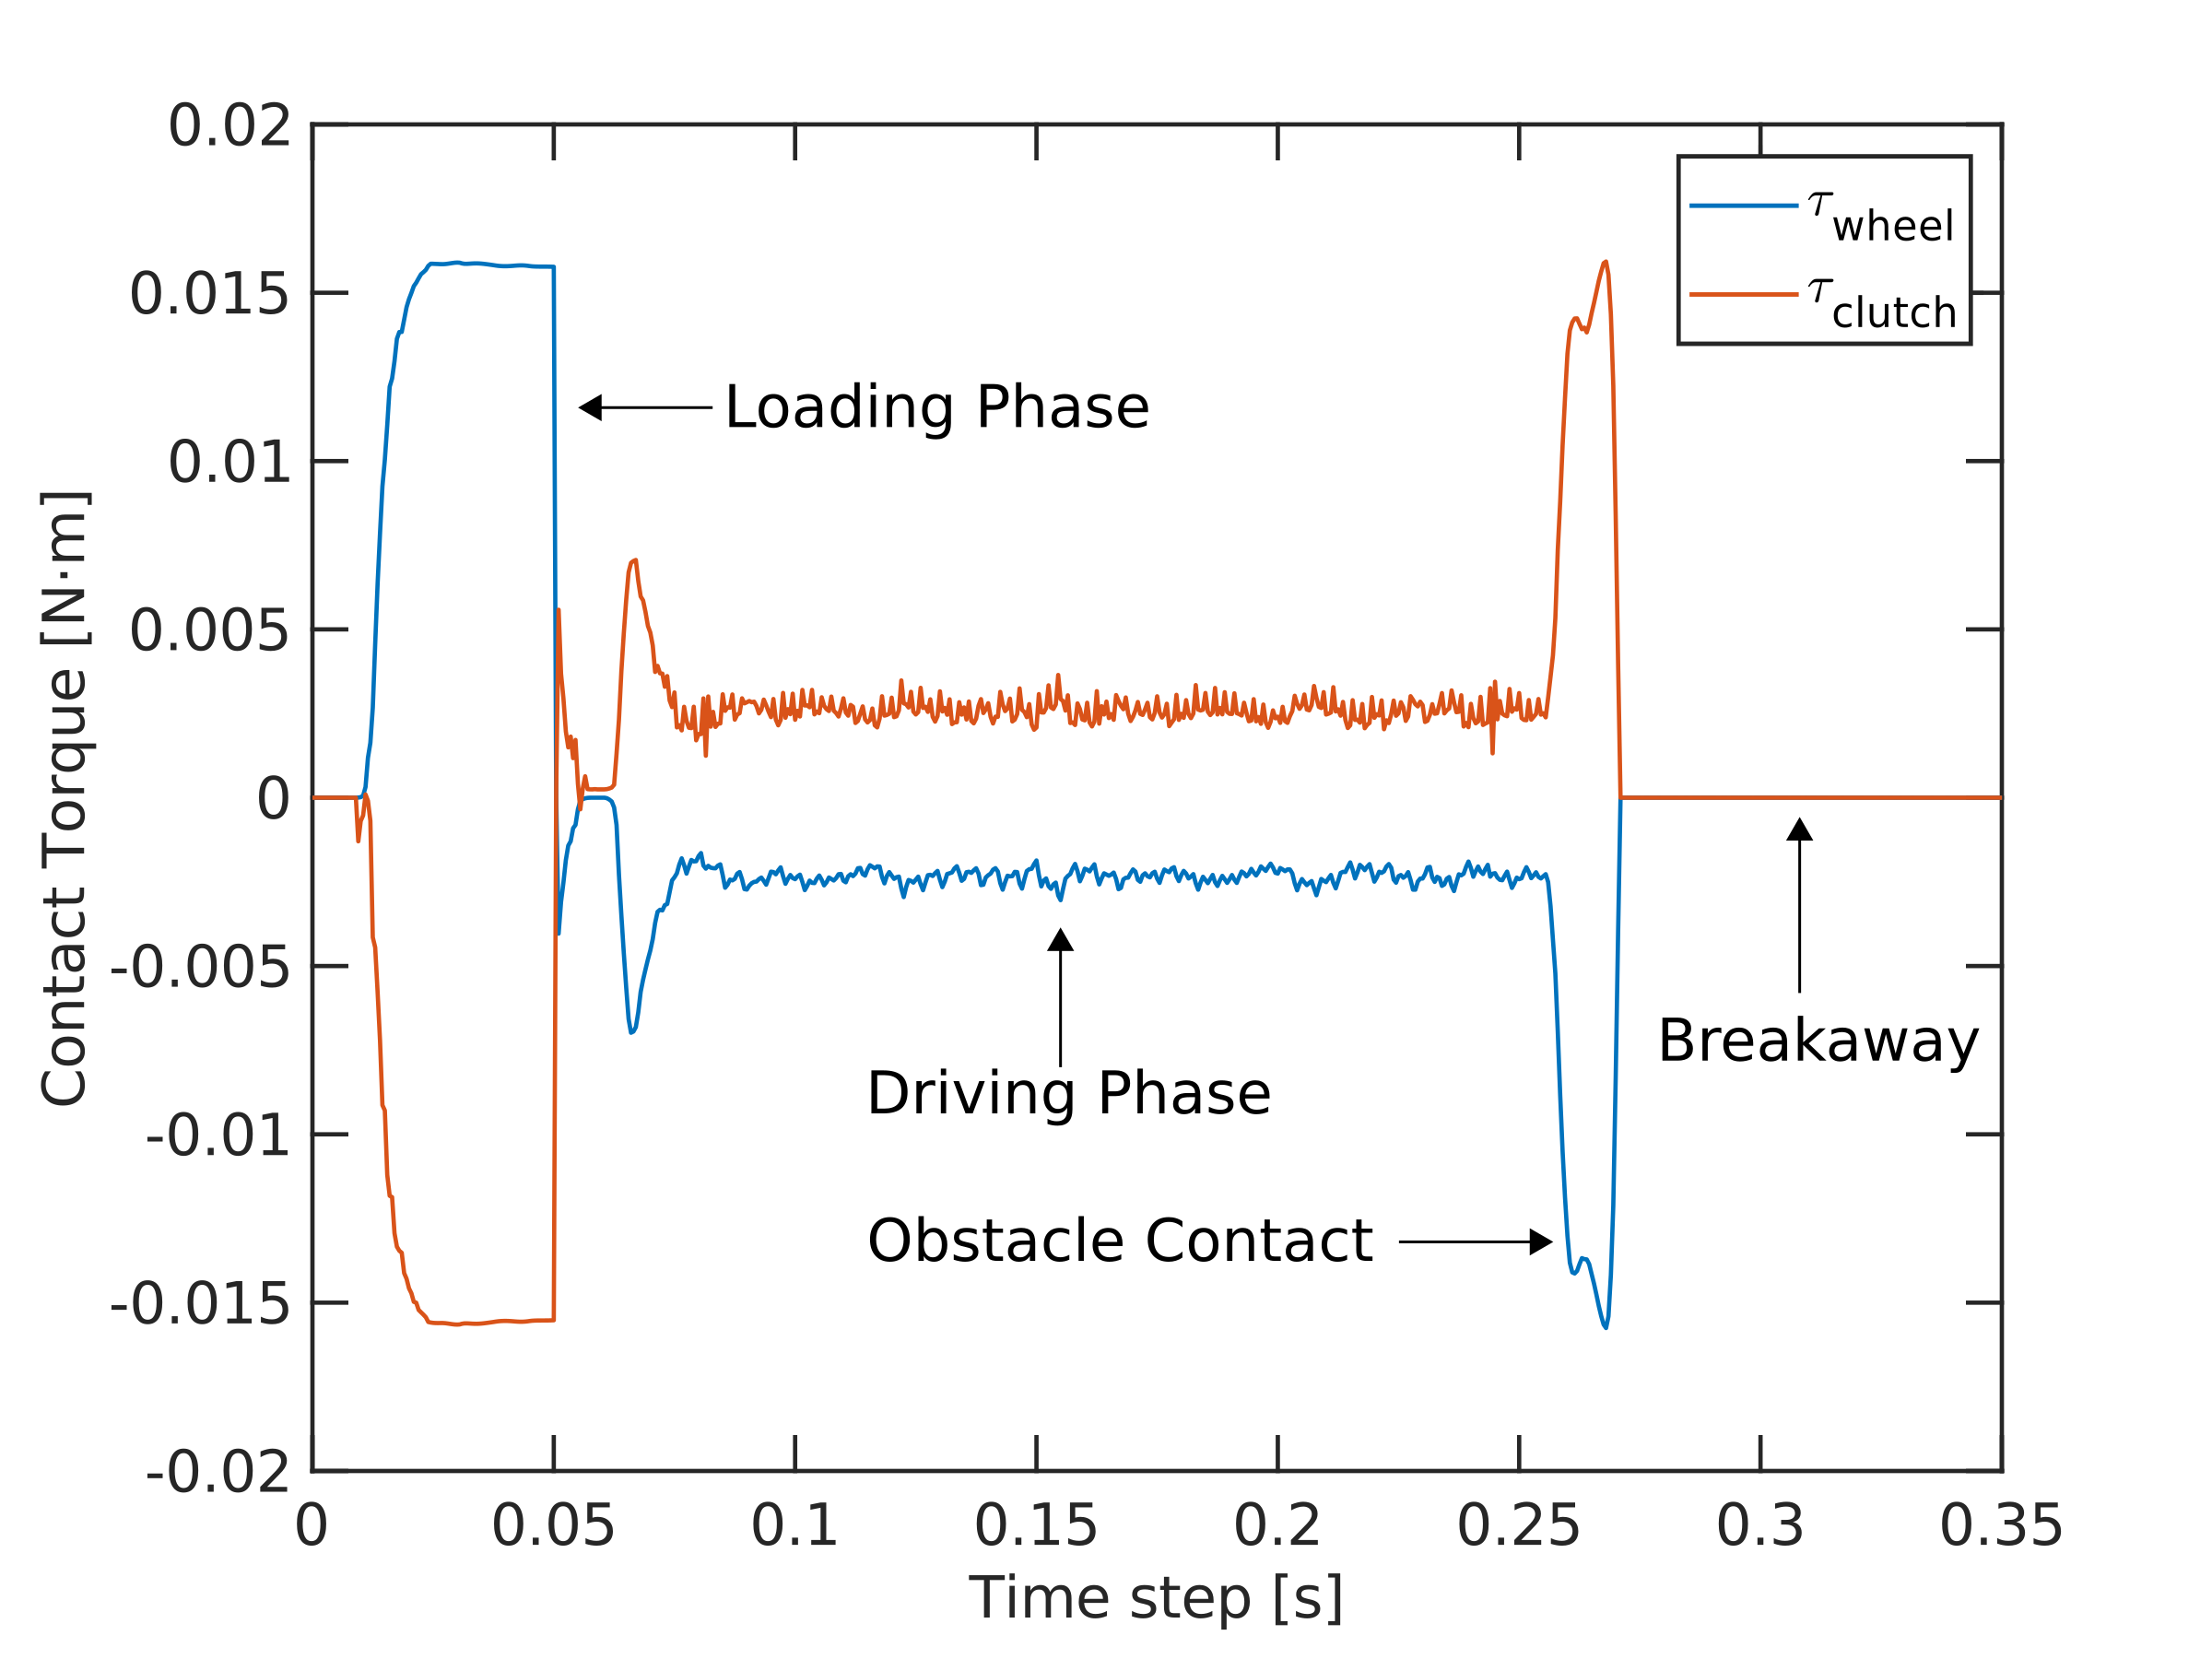
\includegraphics[width=0.9\columnwidth]{figures/TestCases/BarrettHand/contact_torque_annotated.png}
    \caption{Torques on the proximal worm gear transmitted through contact from the proximal wheel and clutch.}
    \label{fig:barrett_torque}
\end{figure}

Finally, we point out that, with the Similar model, we observe a spurious
``locking'' of the proximal wheel's teeth as they glide within the threads of the
worm gear. This is similar to the phenomenon reported in Fig. 2 of
\cite{bib:horak2019}. Therefore, these simulation results use the Lagged model,
which does not introduce any of these artifacts during sliding.
